\begin{task}{1, Principal Component Analysis}

In the implementation we do not use the U and S matrices to recover the data but instead recover the US matrix as shown in the theory part of the assignment (by multiplying with V) and then multiply the US by a diagonal matrix to zero the rows corresponding to the low significance singular values we want to remove. This allows us to use both the procedure used in the theory part of the assignment and also the more commonly used method using the data covariance matrix. It also allows us to generalize the transform and reverse transform operations to arbitrary data.

I created two versions of the implementation, one that calculates the $V^T$ using the centered data matrix decomposition and one that calculates it using covariance matrix decomposition. These methods are very similar except for the fact that their U matrices have different shapes and they produce different eigenvalues and eigenvectors.

\paragraph{1.1: How much energy is contained in each of the two components?}
As we can see in \verb+showcase_PCA.ipynb+ roughly 0.99995 percent is contained in the first component and roughly 0.00005 in the second one.

\paragraph{1.2: Plotting the data and adding the direction of the two principal components}

One thing that caused a measure of confusion was that PCA is usually performed using the SVD of the centered data covariance matrix not the centered data matrix. It seems to be defined like that also in the wikipedia article referenced in the assignment \href{https://en.wikipedia.org/wiki/Principal_component_analysis}{https://en.wikipedia.org/wiki/Principal\_component\_analysis} The covariance (Figure \ref{fig:plot2dPCA}) and centered data matrix (Figure \ref{fig:direct2d}) do not have the same eigenvectors or eigenvalues but both approaches seems to work.

\begin{figure}[H]
    \centering
    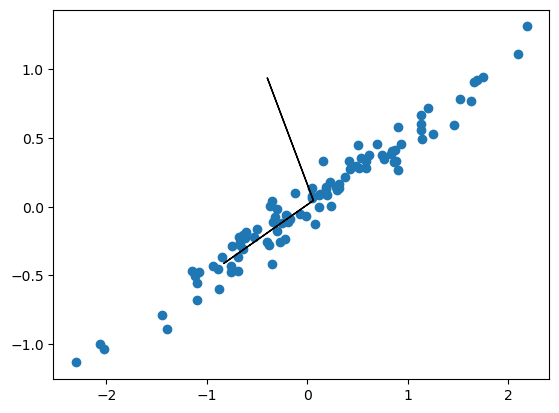
\includegraphics[width=0.8\textwidth]{images/plot2dPCA.png}
    \caption{The showcase data set with the direction of the two principal components when using the covariance matrix method}
    \label{fig:plot2dPCA}
\end{figure}

\begin{figure}[H]
    \centering
    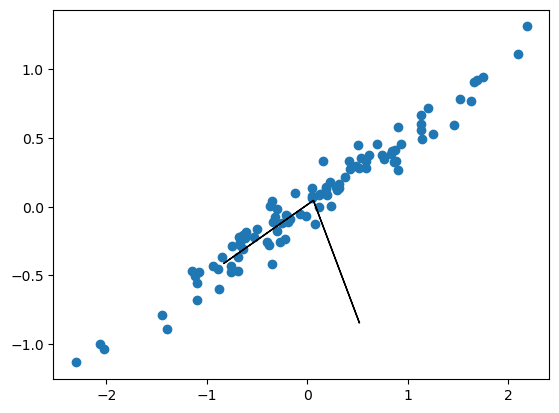
\includegraphics[width=0.8\textwidth]{images/direct2d.png}
    \caption{The showcase data set with the direction of the two principal components when using the data matrix method}
    \label{fig:direct2d}
\end{figure}

\paragraph{2.1: Visualizing reconstructions of the image}

When using many components no change is visible because we are basically just multiplying by something very close to the identity matrix $VV^T$ (Figure \ref{fig:plotImagePCAdirect1}).
When using fewer components the matrix degenerates but the image only seems to degenerate at very low component counts (Figure \ref{fig:plotImagePCAdirect2}).

When we use the covariance method the results are identical (Figure \ref{fig:covar}).

\begin{figure}[H]
    \centering
    \subfigure[all 185 components]{
    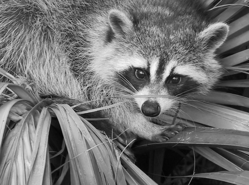
\includegraphics[width=0.45\textwidth]{images/185.png}}
    \subfigure[120 components]{
    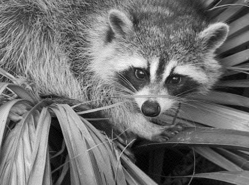
\includegraphics[width=0.45\textwidth]{images/120.png}}
    \caption{The images restored using the procedure in the exercise definition part 1.}
    \label{fig:plotImagePCAdirect1}
\end{figure}
\begin{figure}[H]
    \centering
    \subfigure[50 components]{
    
\includegraphics[width=0.45\textwidth]{images/50.png}}
    \subfigure[10 components]{
    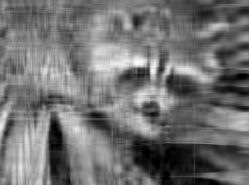
\includegraphics[width=0.45\textwidth]{images/10.png}}
    \caption{The images restored using the procedure in the exercise definition part 2.}
    \label{fig:plotImagePCAdirect2}
\end{figure}
\begin{figure}[H]
    \centering
    \subfigure[50 components]{
    
\includegraphics[width=0.45\textwidth]{images/covar50.png}}
    \subfigure[10 components]{
    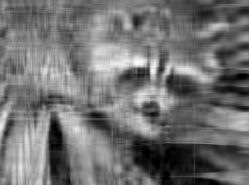
\includegraphics[width=0.45\textwidth]{images/covar10.png}}
    \caption{Image restored using the usual covariance matrix method.}
    \label{fig:covar}
\end{figure}

\paragraph{2.2: At what number is the information loss visible?}

The information loss can be clearly seen only when we use 10 or less components (Figure \ref{fig:plotImagePCAdirect2}). That is because as we will see shortly already at the 9 components the explained variance is more than 99\%. Of course since we are only taking into considerations columns and therefore only 1 dimensional neighbourhood and also doing this non-locally the actual information loss is larger.

\paragraph{2.3 : At what number is the energy lost through truncation smaller than 1\%?}

As can be seen in \verb+picture_PCA.ipynb+ that would be at nine components.

\paragraph{3.1: Visualize the path of the first two pedestrians in 2D space}

Can be seen in Figure \ref{fig:first2pedestriantraj}.

\begin{figure}[H]
    \centering
    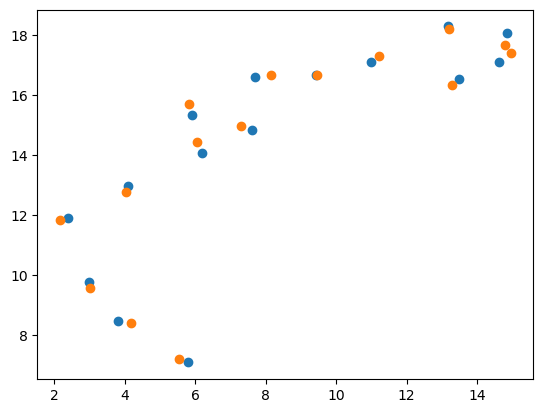
\includegraphics[width=0.75\textwidth]{images/first2pedestriantraj.png}
    \caption{The trajectory of the first two pedestrians}
    \label{fig:first2pedestriantraj}
\end{figure}

\paragraph{3.2: Are two components enough to capture most of the energy of the data set?}

Yes as we can see in \verb+vadere_PCA.ipynb+ the first components whose cumulative sum is greater than 0.9 are the first two.

\paragraph{Part 3.3: Analyze the data set by projecting the 30-dimensional data points to the first
two principal components. Why, or why not? How many do you need to capture most of the energy?}

When using the centered data matrix the L2 between the same pedestrian in the original and recovered space is 1.244. When using the covariance matrix this is instead 4.529, almost three times as much. The embeddings just look differently oriented (Figure \ref{fig:pedestrianembed}).

\begin{figure}[H]
    \centering
    \subfigure[using covariance matrix]{
    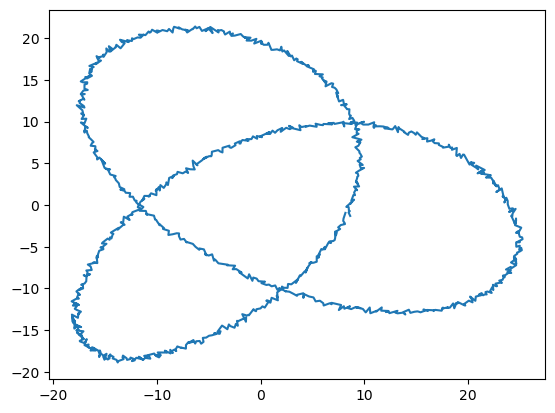
\includegraphics[width=0.45\textwidth]{images/pedestrians_PCA.png}}
    \subfigure[using centered data]
    {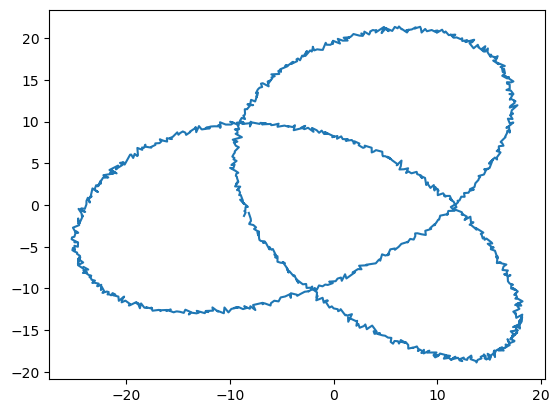
\includegraphics[width=0.45\textwidth]{images/pedestrians_PCA_centered.png}}
    \caption{Embedding the pedestrian trajectories into 2D space.}
    \label{fig:pedestrianembed}
\end{figure}

The first two components are enough because the trajectories of the pedestrians only vary around the mean trajectory in two dimensions.

\paragraph{Answering the three questions from the first page of the exercise sheet}
\begin{itemize}
    \item (a) An estimate on how long it took you to implement and test the method would be about 5 hours.
    \item (b) How accurate could we represent the data and what measure of accuracy you used.
    The average L2 metric between the same pedestrian trajectory in the PCA reconstructed and original data set is about 1.25 (as seen in \verb+vadere_PCA.ipynb+). Since the length of the area in the larger dimension is 30 that seems quite good.
    \item (c) What we learned about both the data set and the method. 
    The data set seems to contain people walking roughly along some curve. PCA works extremely well for data that is only varying in a few directions around some manifold.
\end{itemize}

\end{task}